% !TEX root = ../main.tex

\glsresetall


% \topquote[9cm]{
% \textit{Der Irrsinn ist bei Einzelnen etwas Seltenes, aber bei \\
% Gruppen, Parteien, Völkern, Zeiten die Regel.}
%
% In individuals, insanity is rare; but in \\
% groups, parties, nations, epochs it is the rule.}
% {Friedrich Nietzsche, 1886, \textit{Beyond Good and Evil}}

\topquote[9cm]{%
``Begin at the beginning,'' the King said gravely, \\
``and go on till you come to the end: then stop.''}%
{Lewis Carroll, \textit{Alice in Wonderland}}


\chapter{A deterministic method to detect IBD tracts around rare variants}
\label{ch:sharedhap}
\minitoc





\begin{summary}
In this chapter, I present a new method which capitalises on the presumed young age of rare variants to, first, identify recent relatedness in samples of reportedly unrelated individuals and, second, to detect haplotypes that are identical by descent (IBD) in large sample data.
If an allele is rare, it is likely that the chromosomes carrying that allele are the nearest genealogical neighbours in the sample at that position in the sequence.
A low frequency suggests that the allele was inherited from a common ancestor only a few generations ago, such that recombination had less time to break down the length of the co-inherited haplotype region.
As such, rare variants are utilised as ``bookmarks'' to highlight the positions at which the individuals sharing a focal allele are also likely to share a relatively long haplotype by descent.
The position of a rare allele is used as a target point around which recombination events are inferred along the sequence to both sides of the focal position, which is done in each pair of individuals sharing the target allele.
This approach delimits the region in which the underlying IBD segment is enclosed; \ie the smallest interval detectable from available data in which \n{2} individuals share a haplotype by descent.
Notably, the method presented is non-probabilistic and relies on the observation of certain allelic or genotypic configurations to infer recombination in pairs of diploid individuals.
\N{2} rule-based approaches are implemented which allow the detection of IBD segments in either haplotype or genotype data, respectively.
\end{summary}



%
\section{Introduction}
%


Because all individuals in a finite population are to some degree related,
any point along the genome is identical by descent in \n{2} chromosomes if looking back far enough.

genealogical fragments (\ie marginal trees) along which the relationship status to other chromosomes varies.
Because all individuals in a finite population are to some degree related,
any point along the genome is identical by descent in \n{2} chromosomes if looking back far enough.
 if looking back far enough, any point along their genomes can be traced back to a common ancestor

which may describe a different relations to
stand in a different genealogical relation to other chromosomes in a population.
\ie \n{2} individuals may be separated by a few
but very distantly at the next
Because all individuals in a finite population are to some degree related, if looking back far enough, a random sample of \n{2} chromosomes from the population may reveal some extended regions that are identical by descent.



Over the course of generations, meiotic recombination breaks down
the ``identity'' of the haplotype inherited from a particular ancestor is broken down through recombination,

meiotic recombination
chromosomal rearrangement
maternal and paternal
blending of diverse ancestral lineages


In particular, IBD describes a pairwise relation between the chromosomes of an individual
as meiotic recombination
because recombination rearranges the chromosomes
and thereby blends diverse ancestral lineages
The ancestral ``identity'' of the inherited material is broken down through meiotic recombination over the course of generations,
the relation between any \n{2} chromosomes which derived parts of the genome from this common ancestor

such that the expected length of a pairwise shared \gls{ibd} region is shortened
 \citep[\eg see][]{Browning:2012cx,Thompson:2013cj}.

%, where each segment can be traced back to a founder population at some point in the (recent) past.






Note that most methods do not attempt to scan each pair of haplotypes in large sample data but instead rely on initial ..., so as to limit the computational burden.

Conversely, a larger sample size and higher coverage of the genome facilitate


to make analysis computationally tractable.
A notable example is the
\gls{pbwt}
\citep{Durbin:2014de}

To reduce this search space, it would be beneficial to focus on regions or particular variants that are more likely to sit in recent IBD tracts.
Therefore, in this chapter, a non-probabilistic method is proposed to detect IBD segments around target sites in the genome.
In particular, rare and low-frequency variants are used to identify haplotypes of presumably recent co-ancestry in a larger sample at which it is suggested that
This relation is further explained in the following section.
The variant-centric approach of the method is described in \cpref{sec:ibd_approach}.

the number of rare variants shared between any pair of individuals in a large sample can be informative to reveal patterns of population structure.


In this chapter, I propose a novel method for IBD detection which capitalises on the presumed young age of rare variants to identify (recent) relatedness in samples of reportedly unrelated individuals.

If the allele is rare, it is likely that the chromosomes carrying that allele are the nearest genealogical neighbours in the sample at that position in the sequence.
The low frequency suggests that the allele was inherited from a common ancestor only a few generations ago, such that recombination had less time to break down the length of the co-inherited haplotype region.

The purpose of this chapter is to characterise and test a non-probabilistic method for the detection of shared haplotype segments in large samples, which is based on the classic formulations by \citet{Hudson:1985wh}.
The following section describes the approach by which IBD segments are inferred around selected target sites.
A case is made for the utility of low-frequency or rare variants, as these are likely to optimise IBD discovery.

, as well as to distributions observed in real data, for which the final release dataset of the \gls{1kg} Phase~\rom{3} was used \citep{GenomesProjectConsortium:2012co, 10002015global}.

% TODO extend briefly to shared haplotype sequence inference, in context of overestimation and thereby induced error at edges



%
\subsection{Using rare variants to identify recent IBD}
\label{sec:rarevars}
%


%Alleles which arose recently are more likely to sit in relatively long IBD tracts, as recombination had less time to break down ancestral identity.
%Likewise, because mutations had less time to accumulate along the length of the shared segment, haplotype diversity is expected to be low.

The rate of meiotic recombination is defined as $\si{\Morgan}^{-1}$ where \si{\Morgan} is the unit of genetic distance (\emph{Morgan}).
More commonly, genetic distance is expressed in units of \gls{cM} where ${\SI{1}{\Morgan} = \SI{100}{\centi\Morgan}}$.
On average, ${\SI{1}{\centi\Morgan} \approx 1}$~\gls{Mb} of physical distance in humans \citep{lodish1995molecular}.

% The expected number of recombination events separating $n$ diploid individuals from their \gls{mrca} grows exponentially with the rate of recombination \citep{Ethier:1990ca}.





%and estimate the length of the surrounding IBD region.


To further emphasise the conceptual power of rare variants in the detection of IBD in a large sample, see \cpref{fig:pair_ibd_example} which shows the mosaic of IBD segments shared by \n{2} chromosomes taken from a large simulated dataset (described in \ctref{sec:msprime_sim}).
and the positional distribution of all shared alleles


The proposed method was therefore evaluated by selecting variants at focal sites observed below a low allele frequency threshold.

a focal allele in a sample of $n$ diploid individuals, where $k$ is the number of sharers who are heterozygous for that allele; \ie $k$ refers to allele count and thus frequency in the sample, and where ${1<k<n}$.




% In the following sections, I attempt to demonstrate the utility of rare variants as direct indicators of recent relatedness.
% In particular, I provide examples to show that rare variants are informative to distinguish fine-scale patterns of population structure (\cref{sec:popstruct_1kg}, below), and for the detection of recently co-inherited haplotype segments (\cref{sec:fk_ibd_sim}).




Rare variant sharing is informative for the estimation of fine-scale population stratification structure (),

systematic deviations in allele frequency distributions between population groups due to heterogeneous ancestry backgrounds.


heterogeneous genetic ancestry

refers to systematic differences in ancestry and resulting deviations in allele frequencies among population groups.
Genetic variation is often geographically restricted due to low migration rates
geographically restricted segregation of genetic variation
distinct population groups
Individuals belonging to the same



In the results presented below, I used \gls{pcoa}, also known as classical multidimensional scaling \citep{borg2005}, to visualise the distance among
based on the number of pairwise shared rare alleles.
Using the final release dataset of the \gls{1kg} Phase\rom{3}, I counted the number of rare variants shared between each pair of individuals.
For this, I included all \glspl{snp} observed below $0.5$\% allele frequency.


Note that the data used also contains a small subset of individuals with reported relationship status (\eg parent-and-child trios or duos)



%
%!TEX root = ../../main.tex


\begin{figure}[p]
\centering
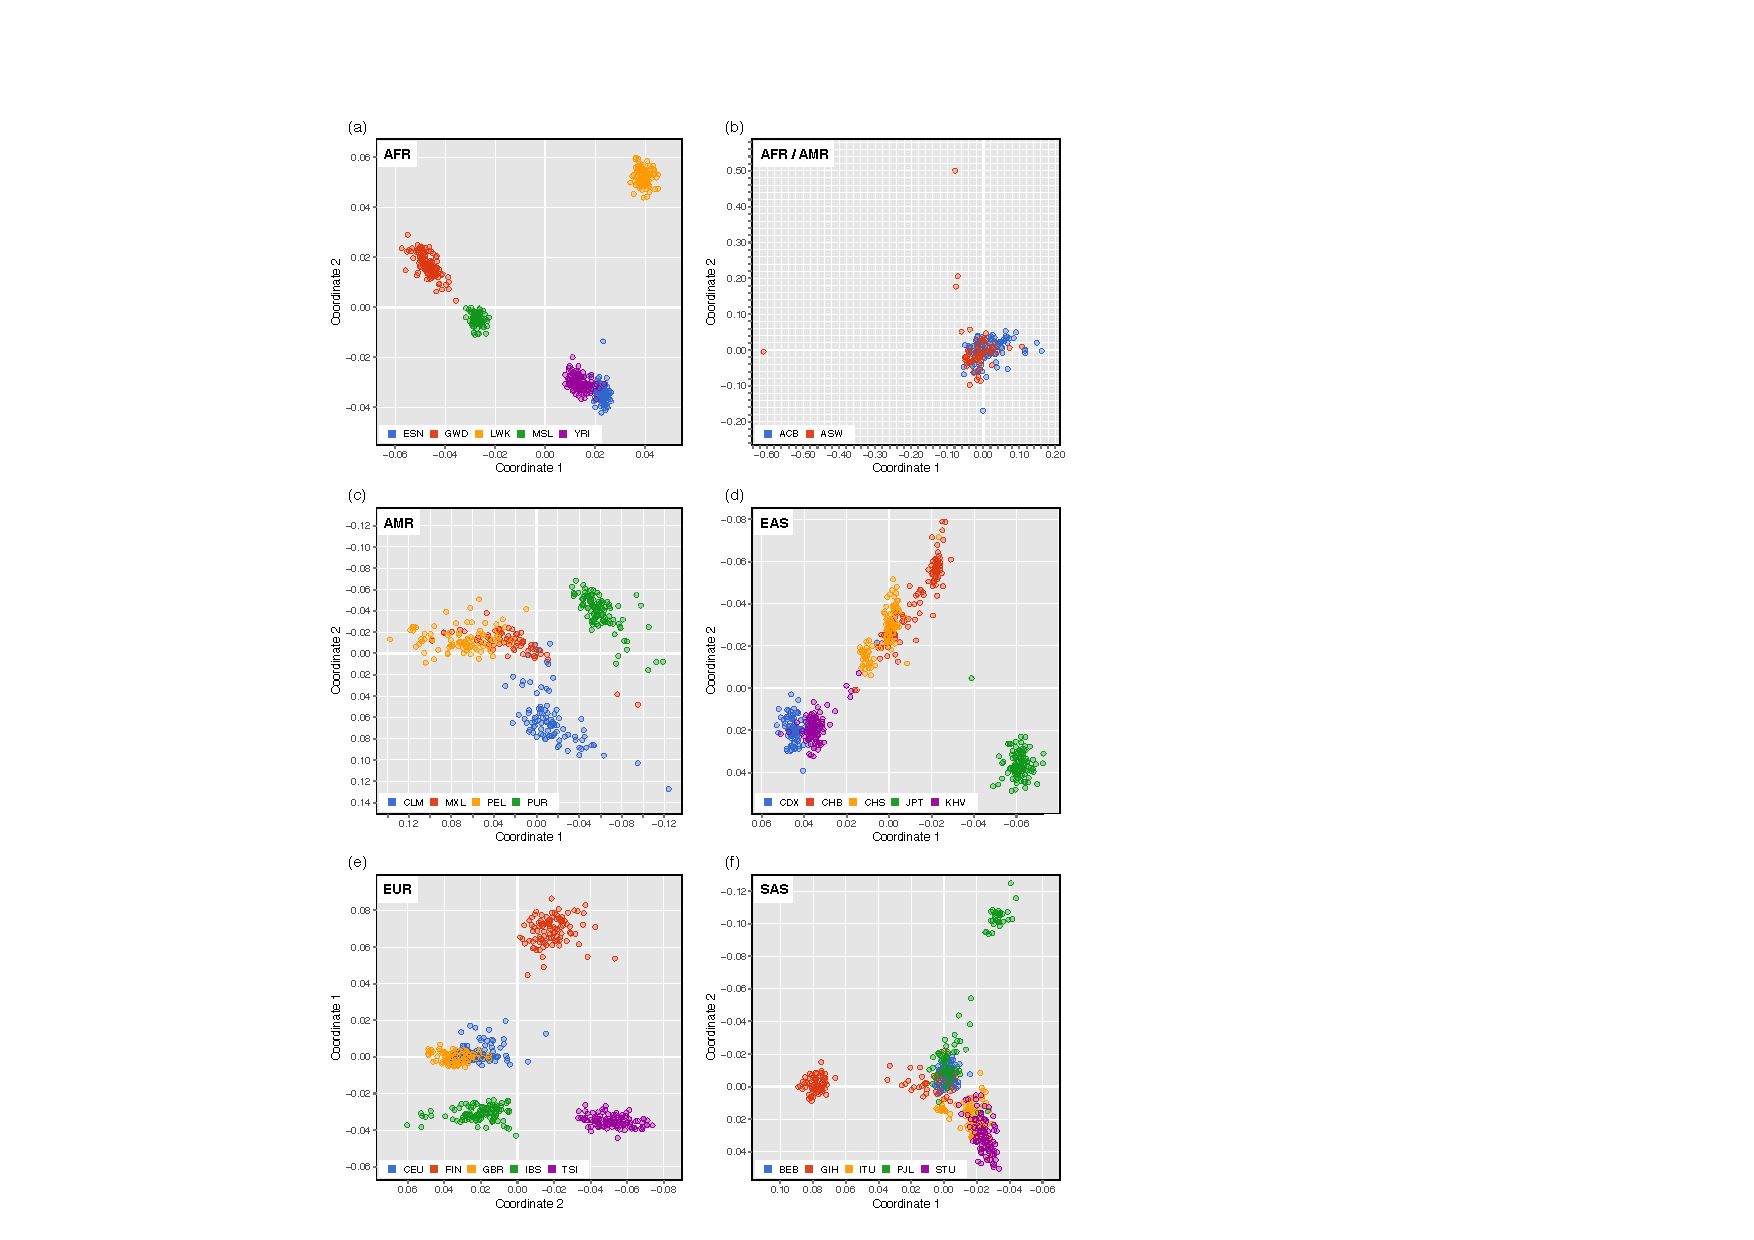
\includegraphics[width=0.9\textwidth]{./img/ch3/pcoa_1kg}
\Caption{Principal coordinates analysis of pairwise shared rare variants}
{...

Axis orientation in each panel was chosen to better reflect the cardinal directions on a geographic map; \ie the top, bottom, left and right sides of each panel roughly correspond to North, South, West, and East, respectively.
Note that the colours used do not adhere to the colour-scheme defined in the \glsentrylong{1kg}; instead, arbitrary colours were chosen to better distinguish population groups.

...}
{fig:pcoa_1kg}
% \vspace{-5pt}
% \hrulefill%
\end{figure}

%






%
\section{Approach}
\label{sec:ibd_approach}
%

\Cpref{fig:info_breakpoint} illustrates how the inference of recombination between \n{2} sites is implemented to detect an IBD segment around a focal site in the genome.

%
\subsection{Inference of recombination events}
%



However, here, because the exact breakpoint of recombination cannot be known from the data, it is therefore represented by a breakpoint interval.


%
%!TEX root = ../../main.tex


\begin{figure}[!htb]
\centering
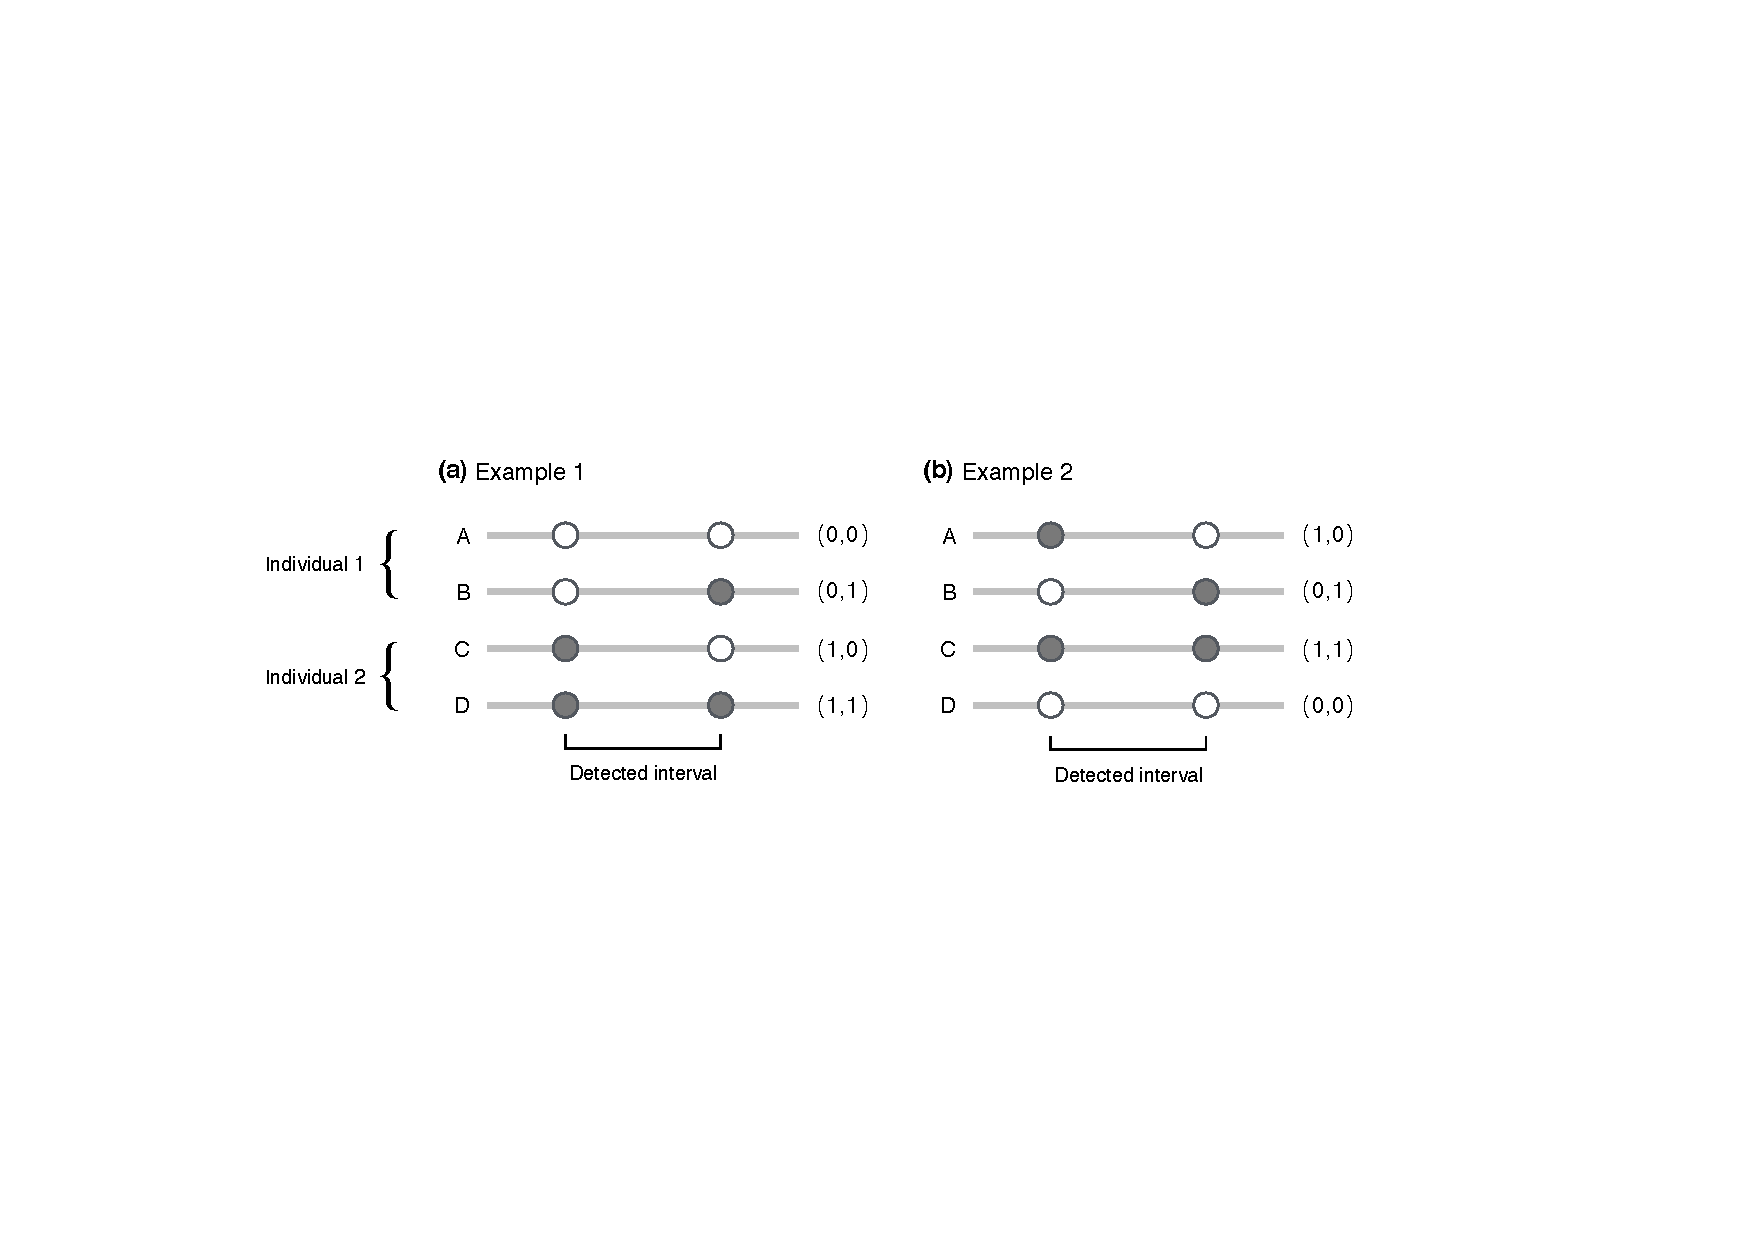
\includegraphics[width=\textwidth]{./img/ch3/info_ibdinterval}
\Caption{Example of allelic configurations satisfying the four-gamete test}
{\N{2} examples are given in which the observation of all \n{4} possible gametes is used to infer a recombination event in the history of the sample, which occurred at some location delimited by the interval spanned between the \n{2} sites.
In particular, both examples are shown with regard to the \n{2}-sample \glsentryfull{fgt}.
The \n{4} gametes (\emph{haplotypes}) are represented by horizontal lines, where ${\{A,B\}}$ belong to Individual~1 and ${\{C,D\}}$ to Individual~2.
The allelic states at the \n{2}~sites are indicated by circles and distinguish between ancestral (\emph{hollow}) and derived type (\emph{solid}).
The corresponding allelic configurations, as used in notation, are given to the \emph{right} of each gamete.
Note that all \n{4} possible gametes are found in both examples, where only their order and occurrence in individuals differ.}
{fig:info_ibdinterval}
% \vspace{-5pt}
% \hrulefill%
\end{figure}

%










%
\subsection{Shared haplotype discovery in multiple individuals}
\label{sec:naive_algorithm}
%







By performing pairwise searches over all sharers (\ie individuals sharing the focal allele), an approximate profile of the recombination history in the sample is reconstructed.

Because recombination events occur at random positions in the DNA sequence (following a Poisson process), detected breakpoints may differ among sharer pairs, but may also be identical, for example, if individuals are separated by only few meioses, or if several recombination events occurred within the same interval.
The latter would not be distinguishable from the data.

In any pair, a given breakpoint interval may be detectable from multiple focal alleles which may or may not share the same local history.

In the following, the term \emph{shared haplotype} is used to refer to the \emph{detected} breakpoint interval around a focal site in a pair of individuals, which is distinguished from actual IBD, referring to the underlying haplotype block that is identical by descent.

Because chromosomes may not recombine at sites that segregate in the sample, the first sites observed after the nearest recombination points (distal from the focal position) are defined as \emph{true} IBD breakpoints.
This interval sets the benchmark to evaluate IBD discovery, as it represents the smallest interval around the recombination points in the sequence of observed variant sites.


A potential caveat of using rare variants to identify recent haplotype sharing  is the dependency on sample size.
If the number of individuals is too small, it becomes less likely that an allele marked as being ``rare'' is actually rare in the population.
A large sample size is therefore recommended.


%
\subsection{Anticipated limitations of this method}
\label{sec:ibd_limits}
%

% TODO write about older variants sitting in younger interval

As noted by \citet{Hudson:1985wh}, not all recombination events in the history of a sample are detected by the \gls{fgt}; for example if the sample size is small.
% TODO lookup why in Hudson 1985
For example, \n{2} sites between which a recombination event occurred at some time in the past in the history of the sample may not satisfy the breakpoint condition.
However, because intervals are found by scanning outward from the focal site, it is likely that breakpoints are found eventually.
This more so applies to the \gls{dgt}, as the number of arrangements which satisfy the breakpoint condition is lower.
Boundary cases may therefore be encountered, even if recombination has occurred.



%%!TEX root = ../../main.tex

\begin{figure}[!htb]
\begin{center}
\begin{tikzpicture}[<->,>=stealth,auto,node distance=3cm,thick,
CHR/.style={circle,draw,thick,minimum size=0.8cm,font=\sffamily\bfseries},
IDV/.style={rectangle,draw=gray,thick,inner sep=6mm}]
\node[CHR,fill=Ivory2] (1) {1};
\node[CHR,fill=Azure2] (2) [right of=1] {2};
\node[CHR,fill=Ivory2] (3) [right of=2] {1};
\node[CHR,fill=Azure2] (4) [right of=3] {2};
\node[IDV,label={[font=\sffamily]below:Individual A},fit=(1) (2)] {};
\node[IDV,label={[font=\sffamily]below:Individual B},fit=(3) (4)] {};
\draw [<->] (1) to [out=18,in=162] (2);
\draw [<->] (1) to [out=36,in=144,looseness=0.666] (3);
\draw [<->] (1) to [out=54,in=126,looseness=0.666] (4);
\draw [<->] (2) to [out=18,in=198] (3);
\draw [<->] (3) to [out=342,in=198] (4);
\draw [<->] (2) to [out=324,in=216,looseness=0.666] (4);
\end{tikzpicture}
\end{center}
\Caption{Illustration of the possible shared haplotypes in two individuals}
{what the hell is going on here. i have no idea!}
{fig:six_chrom_pairs}
% \Caption{Illustration of the possible shared haplotypes in two individuals}
% {Given \n{2} diploid individuals, each of the \n{4} chromosomes may share a haplotype identical by descent.}
% {Given \n{2} diploid individuals, each of the \n{4} chromosomes may share a haplotype identical by descent.
% As such, it is possible that the inferred IBD regions may overlap.}
% {fig:six_chrom_pairs}
% \vspace{-5pt}
% \hrulefill%
\end{figure}
 % caption not working, figure redundant





% However, it has been argued that the infinite sites model
% the number of variant sites in a sample is small compared to the number of sites in the nucleotide sequence of the genome
% mutation rate
% \citep{hein2004gene}




%
\section{Evaluation using simulated data}
\label{sec:evalsimdata}
%

In this section, I describe how data were simulated and then used
first, the generation of both haplotype and genotype data using coalescent simulations.
These were carried out under a realistic demographic model

Note that the IBD detection results obtained in other parts of this thesis (\eg Chapter~4) will also follow the same procedure as outline in this section.


%
\subsection{Coalescent simulations}
\label{sec:msprime_sim}
%


%
\subsubsection{Demographic model}
%

%
%!TEX root = ../../main.tex


\begin{figure}[!htb]
\centering
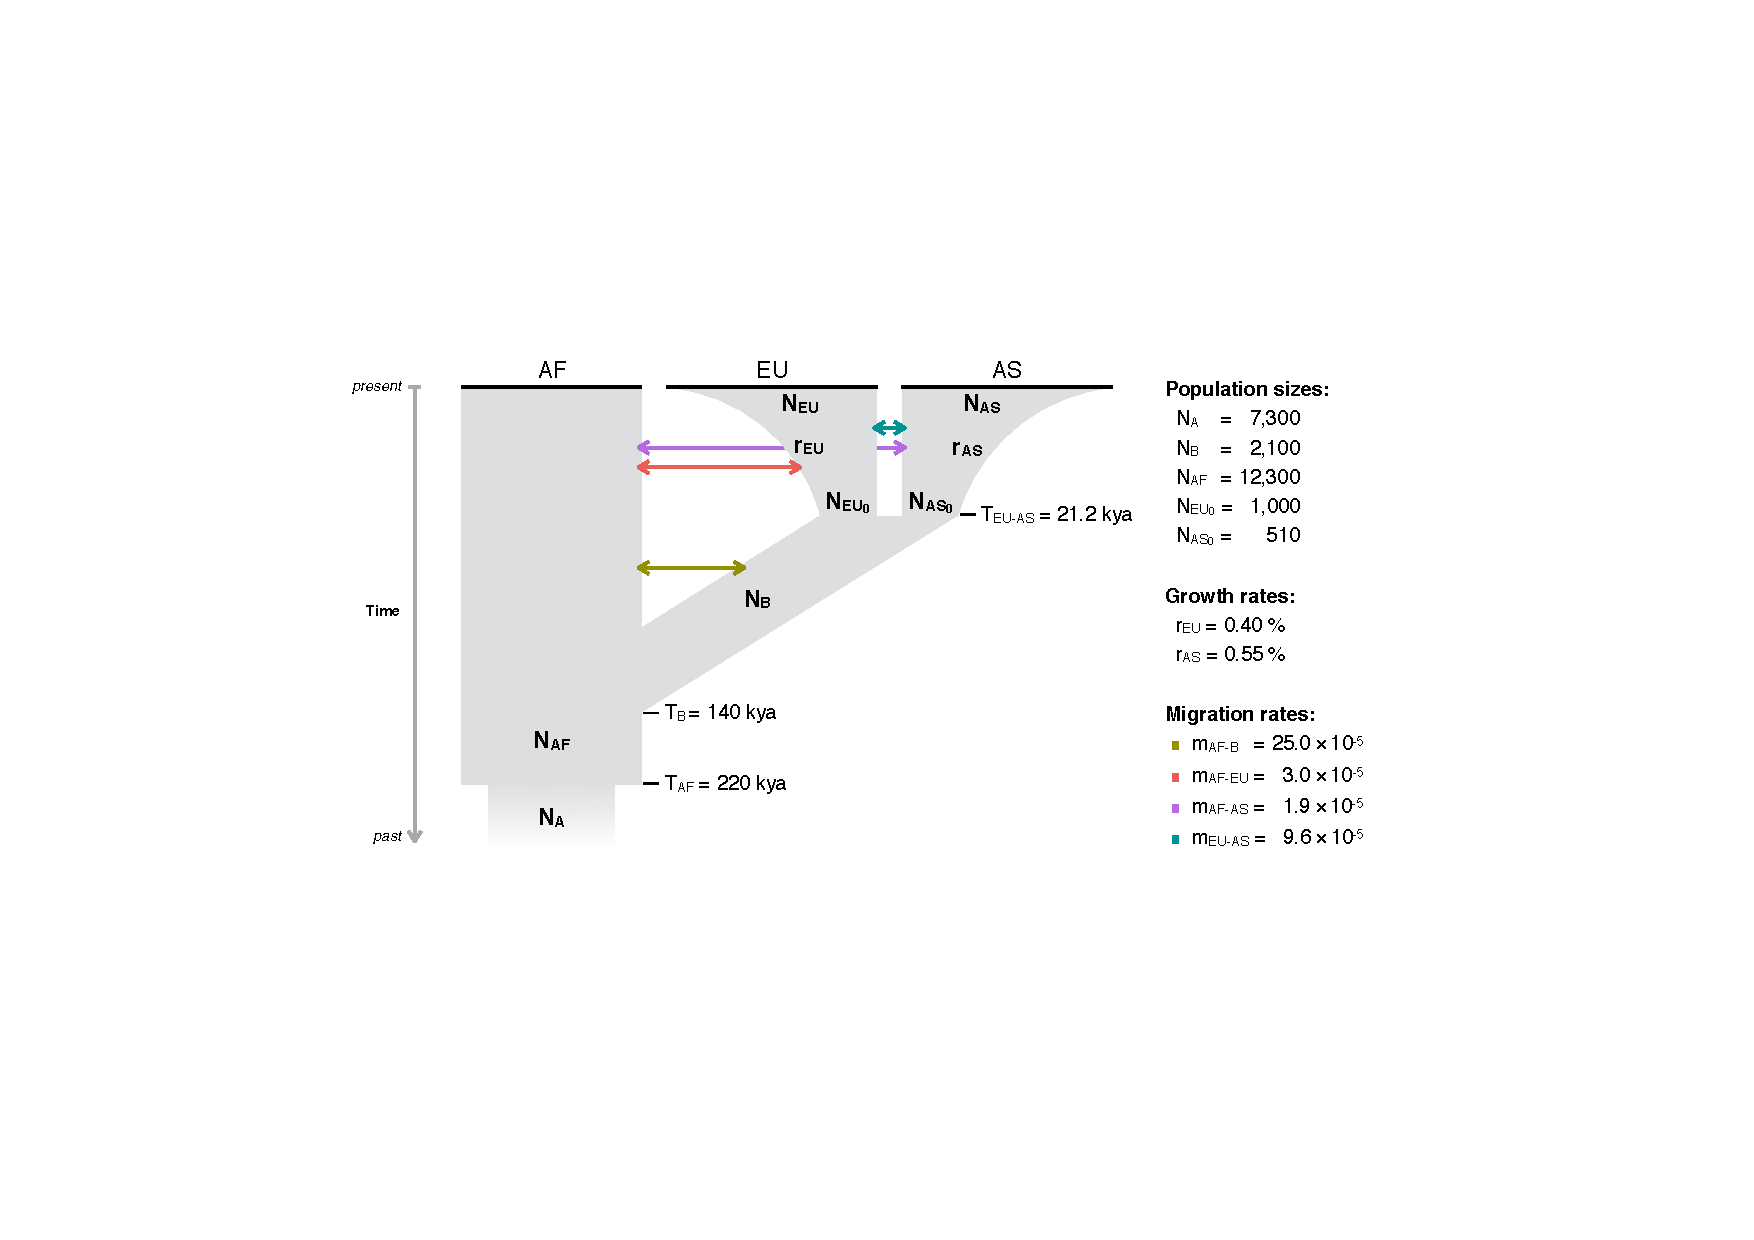
\includegraphics[width=0.95\textwidth]{./img/ch3/demo_model}
\Caption{Demographic model used in simulations}
{\N{3} populations were modelled, African (AF), European (EU), and Asian (AS), which derive from an ancestral population (A).
Both EU and AS experienced a bottleneck with subsequent exponential growth following the out-of-Africa expansion of a founder population (B) that split from the ancestral population.
Modified from \citet{Gutenkunst:2009gs}, Figure~2 (see \url{doi:10.1371/journal.pgen.1000695.g002}), with parameter values taken from Table~1 (see \url{doi:10.1371/journal.pgen.1000695.t001}).}
{fig:demo_model}
% \vspace{-5pt}
% \hrulefill%
\end{figure}

%

The demographic model used for simulations followed \citet{Gutenkunst:2009gs}, who used intergenic data from \n{4} \gls{hapmap} populations (YRI, CHB, EUR, and MXL) to estimate parameters from diffusion approximations of expected allele frequency spectra.
Accordingly, simulations were carried out with an effective population size of ${N_e = \num{7300}}$ and under the assumption of a generation time of 25 years.
The mutation rate was set to a constant ${\mu = \num{2.35e-8}}$ per site per generation, which was estimated from the human-chimp divergence in \citet{Gutenkunst:2009gs}.
Note that more recent studies have estimated the human mutation rate to be slightly lower; for example, \citet{Scally:2012fe} have estimated ${\mu \approx \num{1.2e-8}}$ from analyses of genome-wide \emph{de~novo} mutations using recent sequencing technologies, but which is in the same order as the mutation rate defined here.
\Cpref{fig:demo_model} illustrates the demographic history as defined in the simulation model (all parameter values of the simulation model are specified therein).
The model recapitulates the human expansion out of Africa, for which \n{3} populations were considered; African (AF), European (EU), and Asian (AS).
The African population was included with a constant population size, while EU and AS experienced exponential growth after divergence and split from an ancestral African population.
Population sizes of EU and AS were calculated as ${N = \rfrac{N_0}{\euler{-r t}}}$, where $N$ is the size at present, $N_0$ the initial size at EU-AS divergence, $r$ the growth rate, and $t$ the time since divergence (in years).





%
\subsubsection{Accuracy analysis}
\label{ibd_accuracy}
%






%
\subsection{Results}
\label{ibd_results}
%




%
%\subsection{Conclusions}
%


%
\section{Haplotype estimation and genotype phasing from detected IBD segments}
%

Recent advances in high-throughput genotyping and sequencing technologies have made it possible to obtain genotype data for more efficient and cost effective to produce genotype data for large samples.

Statistical phasing of genotype data has become a fundamental problem in genetic research \citep{Browning:2011ic} and

Enormous amounts of genotype data are being generated

Due to the recent advancements in genotyping and \gls{ngs} technologies
% recent growth in genetic datasets, yield genotype data
% phasing is crucial in many applications
% many methods require or would benefit from haplotype information
% large body of literature is devoted to relatedness
% if pedigree-based, limitations as defined by the Lander-Green algorithm
% computational complexity, efficiency, and time
% the most accurate methods use HMMs, either with or without reference (if large enough)
% however, accuracy of rare variants is lagging behind


Statistical phasing of genotype data
estimation of haplotypes from genotypes is a crucial step

While there are recent technologies that attempt to generate haplotype information along chromosomes,
high-throughput genotyping or sequencing methods are typically designed to produce genotype data

For example, the Lander-Green algorithm \citep{Lander:1987vc}


Because many analytical methods either require or would benefit from haplotype information


\citep{Browning:2011ic}
As with the discovery of IBD segments,

Statistical methods for haplotype phasing address a key problem in genetic analysis and are a crucial step
is a crucial step in many methods for genetic data analysis

In this section, I explore the feasibility to use IBD information obtained from rare variant sharing by descent to deduct the sequence of the underlying shared haplotype within a given breakpoint interval of a detected IBD segment.
Thus, this analysis attempts to
a \emph{local} phasing approach
Since it assumed that the

The presented approach is non-probabilistic and follows a set of rules to determine the allelic state shared between \n{2}~individuals.

Since the \gls{fgt} already assumes haplotype information, IBD segments are detected using the \gls{dgt}.

\citep{Kong:2008gh}



IBD information is expedient to determine the underlying haplotype sequence that is shared between \n{2} individuals and, hence, to distinguish haplotypes from genotype information.

Current genotyping or sequencing technologies typically produce genotype data.
On the other hand, statistical methods for genetic analyses require
a phasing step in which haplotypes are statistically inferred from genotypes.

The purpose of this section is to

in \n{2} regards;
first, to explore the effect of overestimation of the true IBD segment
second, to explore the ability to distinguish the \n{2} chromosomes in each individual



%
\subsection{Inference of the shared allele}
%



; see the advice on overestimation in \cpref{sec:ibd_limits}.
Hence, it is expected that
The quantification of such error is the focus of the analysis presented

it is possible to deduce the sequence of the shared haplotype


If both individuals are heterozygous at a given site, haplotype phase cannot be resolved from IBD constraints alone, as it cannot be distinguished whether

Note that this caveat is similar to the Lander-Green algorithm which is unable to phase sites at which all members of the pedigree are heterozygous.


Note that the purpose of this chapter is to demonstrate the utility of rare variants as indicators for relatedness.
In that regard, this section provides ...
However, it should be noted that the main focus pertains the development of an IBD detection method.




%
%!TEX root = ../../main.tex


\begin{figure}[!tbp]
\centering
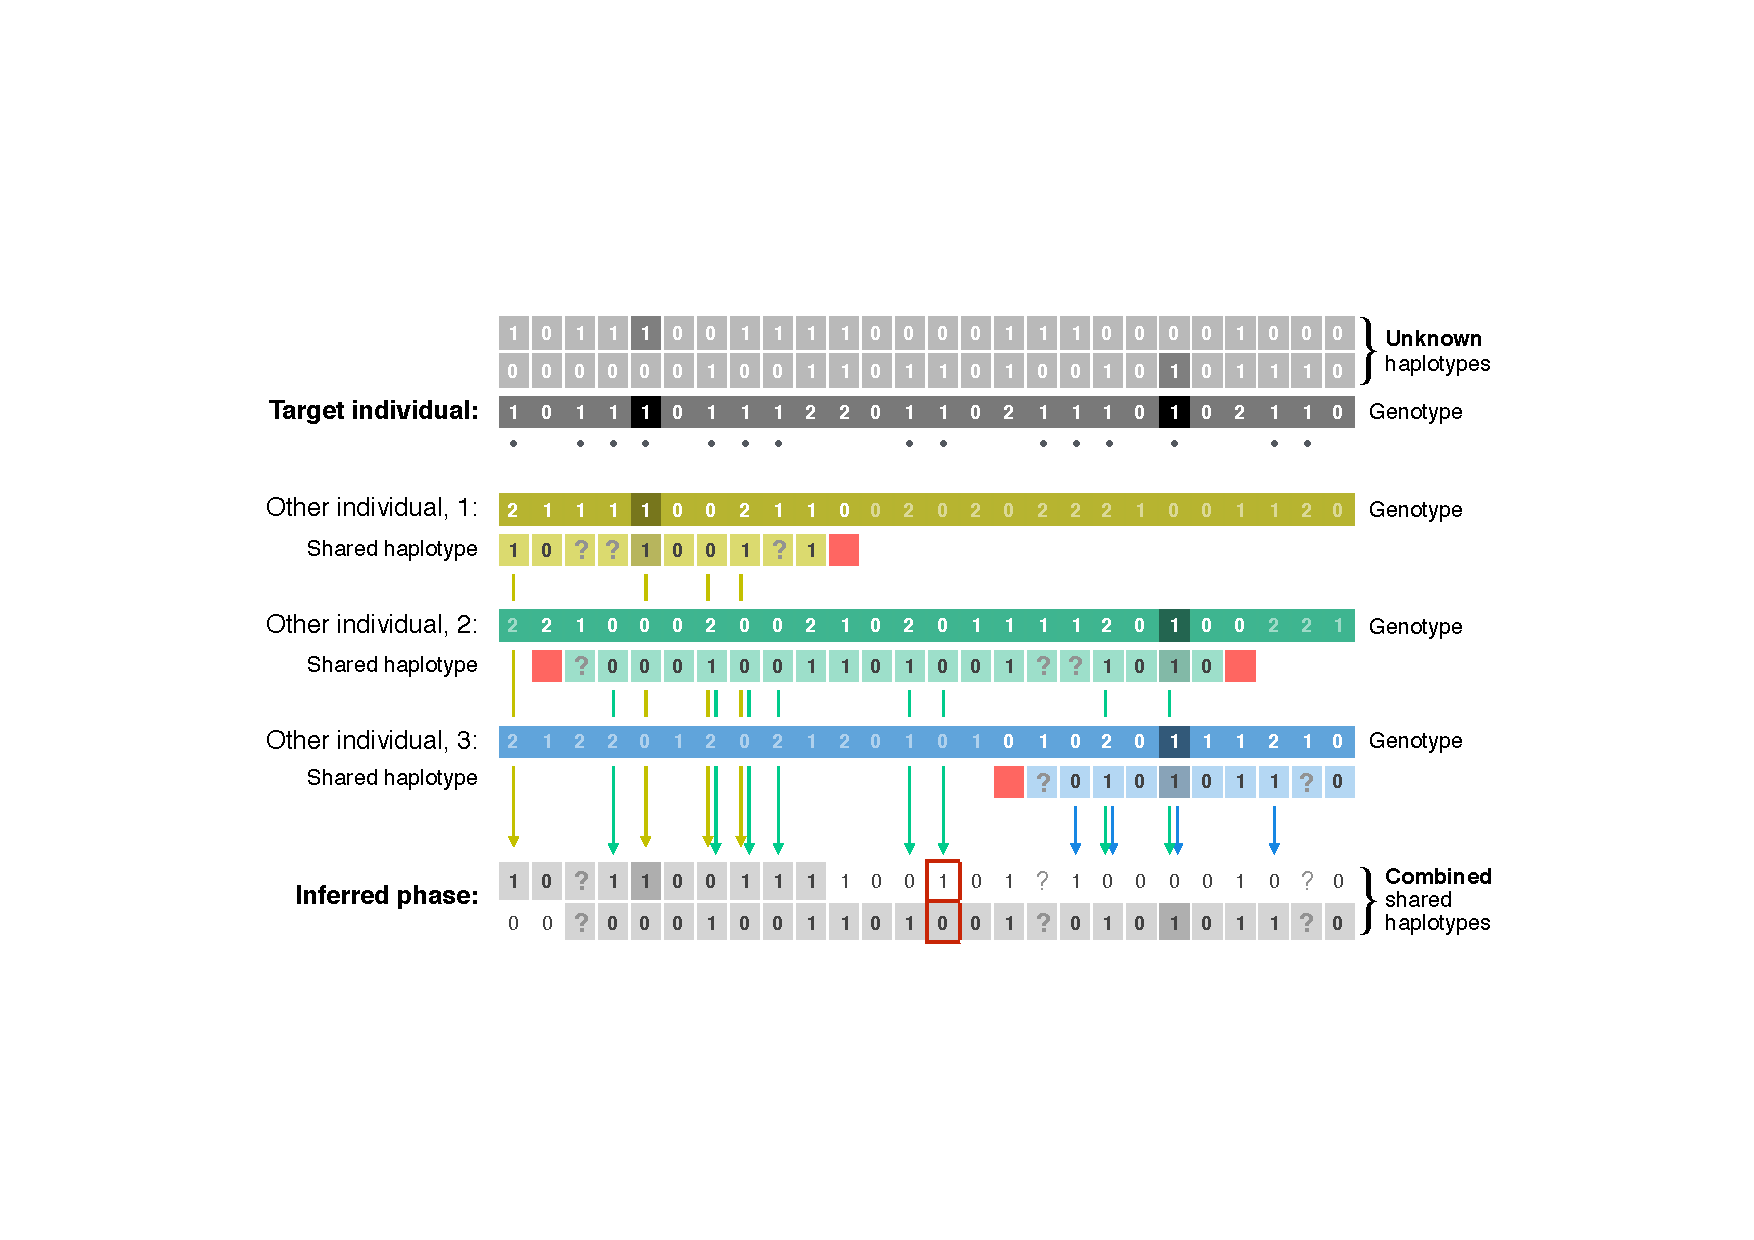
\includegraphics[width=\textwidth]{./img/ch3/info_ibdphasing}
\Caption{Illustration of genotype phasing using detected IBD segments}
{...
% TODO complete caption
Dots below the target genotype indicate heterozygous sites, at which haplotype phase is unknown; haplotypes are already known at homozygous sites, as both haplotypes carry the same allele.

Breakpoints are excluded from inference, because the haplotype cannot be shared at breakpoint positions (\emph{red} blocks).

At positions where both genotypes are heterozygous, the shared haplotype cannot be inferred; indicated by \emph{``?''}.
Note that phase may not be resolved at all sites, even after combination of inferred segments.
Also, singletons may not be phased correctly using this approach; this is illustrated in the figure (\emph{red} outline in inferred phase).}
{fig:info_ibdphasing}
% \vspace{-5pt}
% \hrulefill%
\end{figure}

%


%
%!TEX root = ../../main.tex


\begin{figure}[!htb]
\centering
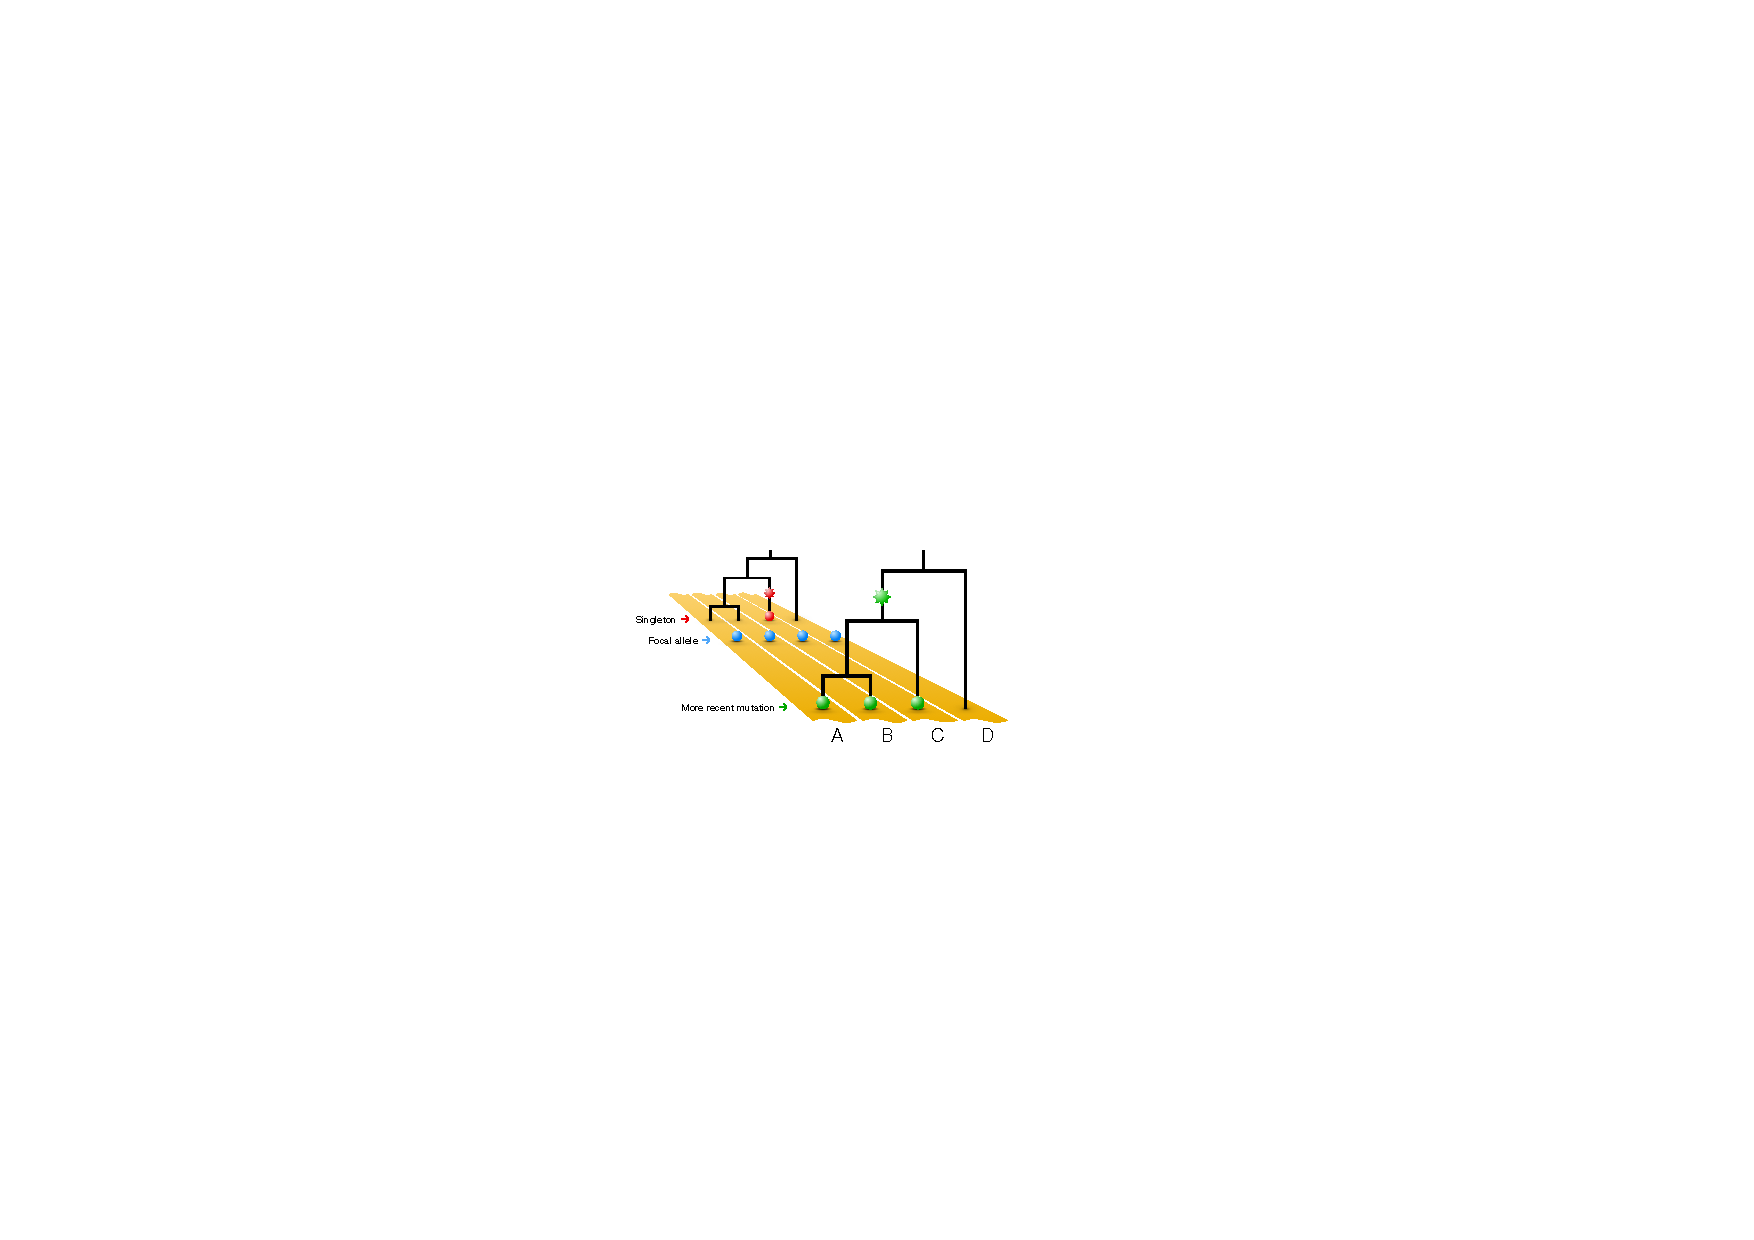
\includegraphics[width=0.9\textwidth]{./img/ch3/info_phase_incons}
\Caption{Illustration of genealogical shared haplotype inconsistency}
{A sample of \n{4} haplotypes is shown which correspond to the haplotype regions that are identicial by descent in \n{4} individuals; \emph{A}, \emph{B}, \emph{C}, and \emph{D}.
The shared haplotype is identified by a focal allele~(\emph{blue}).
Note that there is only \n{1} genealogical tree connecting the \n{4} haplotypes over the region shown; as such, the \n{2} shown trees have the same topology and branch lengths.
In this example, each tree marks the chromosomal position of a genetic variant (not shown for the focal variant), where alleles~(\emph{balls}) derive from mutations~(\emph{stars}) as indicated on each tree.
On the left-hand side, the tree shows a private mutation (singleton) which leads to the observation of the derived allele (\emph{red}) on the shared haplotype in individual \emph{C}.
The tree on the right-hand side shows a mutation that occurred more recently than the mutation that gave rise to the focal allele.
Because it is more recent, the derived allele (\emph{green}) can only be observed in haplotypes in a subtree; \ie the shared haplotypees in individuals \emph{A}, \emph{B}, and \emph{C} in this example.}
{fig:info_phase_incons}
% \vspace{-5pt}
% \hrulefill%
\end{figure}

%



%
%!TEX root = ../../main.tex


\begin{figure}[!htb]
\centering
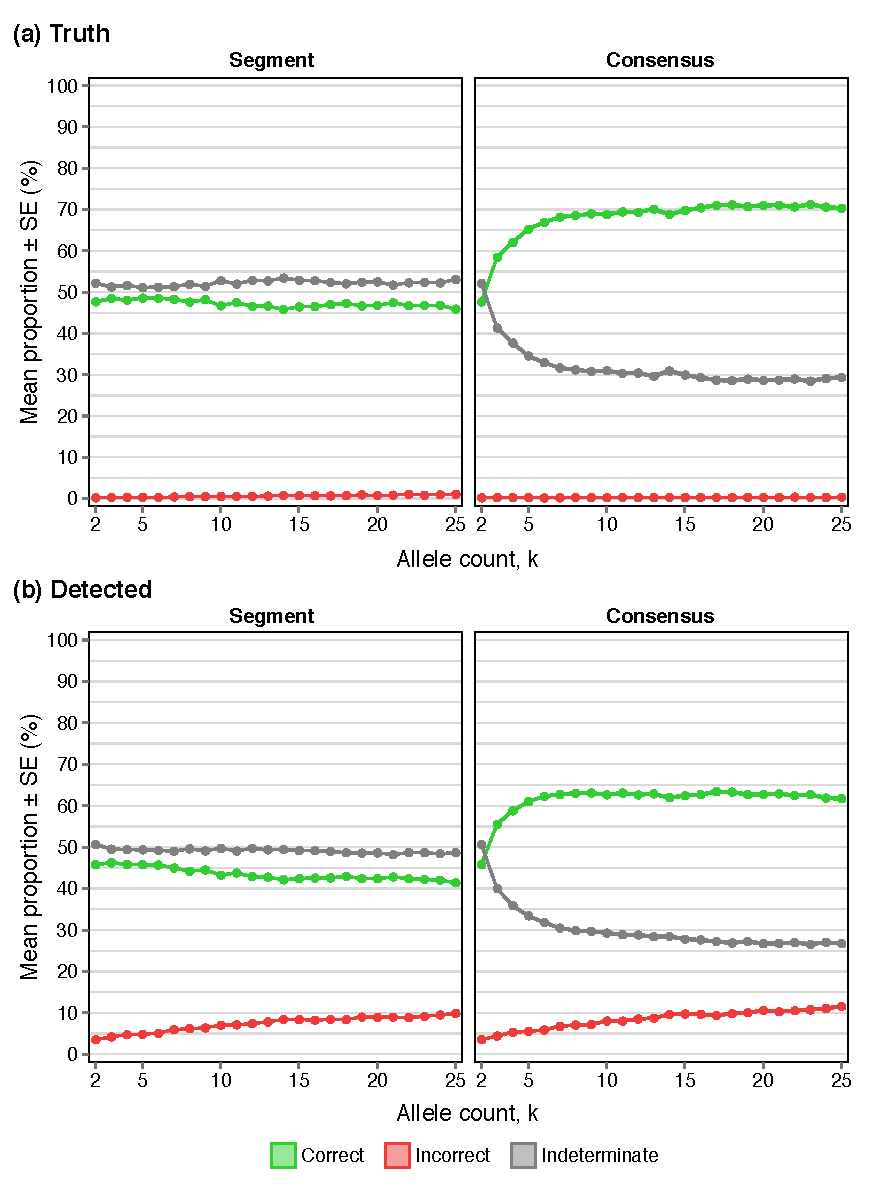
\includegraphics[width=0.75\textwidth]{./img/ch3/phase_fk_prop}
\Caption{Accuracy of alleles inferred through IBD-based phasing by focal allele frequency}
{IBD segments were randomly selected; \n{10000} per \fk{}~category.
Genotypes within each segment were phased and the relative proportions of correct, incorrect, and indeterminate alleles were recorded and averaged ($\pm\text{SE}$) per \fk{}~category.
This was done separately per segment (\emph{left}) and using the consensus approach (\emph{right}).
The results shown in Panel~\textbf{(a)} correspond to the ``truth'', where the true IBD segments were used to delimit the extent of the inferred shared haplotype sequence.
This is compared to Panel~\textbf{(b)}, where the \gls{dgt} was used to detect IBD breakpoints in genotype data.}
{fig:phase_fk_prop}
\end{figure}

%




Several quantities are of interest to determine the feasibility of using rare variant information for genotype phasing.
-- coverage per target individual
-- accuracy of the inferred shared haplotype
-- amount of indeterminant alleles











%
\section{Comparison to shared haplotypes detected in real data}
\label{ibd_1kg_results}
%

Evaluations so far have been based on inference from simulated data.
However, it is not far to seek confirmation by comparison to real data.
Therefore, in this section, the distribution of inferred shared haplotype lengths is investigated in data from the \glsentrylong{1kg} \citep{GenomesProjectConsortium:2012co,10002015global}.
The dataset comprises 84.4~million variants, of which 78~million are \glspl{snp}, identified in a sample of \n{2504} individuals from \n{26} populations across \n{5} continental populations.
Samples were sequenced at low coverage, to a depth of 2-4x, and genotype data were phased using \tagname{SHAPEIT\,2}.
Hence, \cref{app:fgt_p,app:dgt} were carried out as described in the previous section \cref{app:fgt_p,app:dgt}.

Across autosomes 1-22, a total of \gap~million \fk{} variants was selected, at ${k \in \lbrace 2, \ldots, 25 \rbrace}$, which included all \glspl{snp} found at allele frequency between 0.04\% and 0.5\%.
From those, 14~million focal sites were identified around which breakpoint intervals were detected in each approach.
The number of segments retained after removing boundary cases and retaining unique segments only was 9.154~million in \cref{app:fgt_p} and 8.763~million in \cref{app:dgt} over all chromosomes.

As true IBD regions cannot be known, the following analysis focused on the distribution of shared haplotype lengths, which was compared to theoretical expectations.




%
\subsection{Rare variant sharing in the 1000 Genomes dataset}
%


%
%!TEX root = ../../main.tex


\begin{figure}[p]
\makebox[\textwidth][c]{%
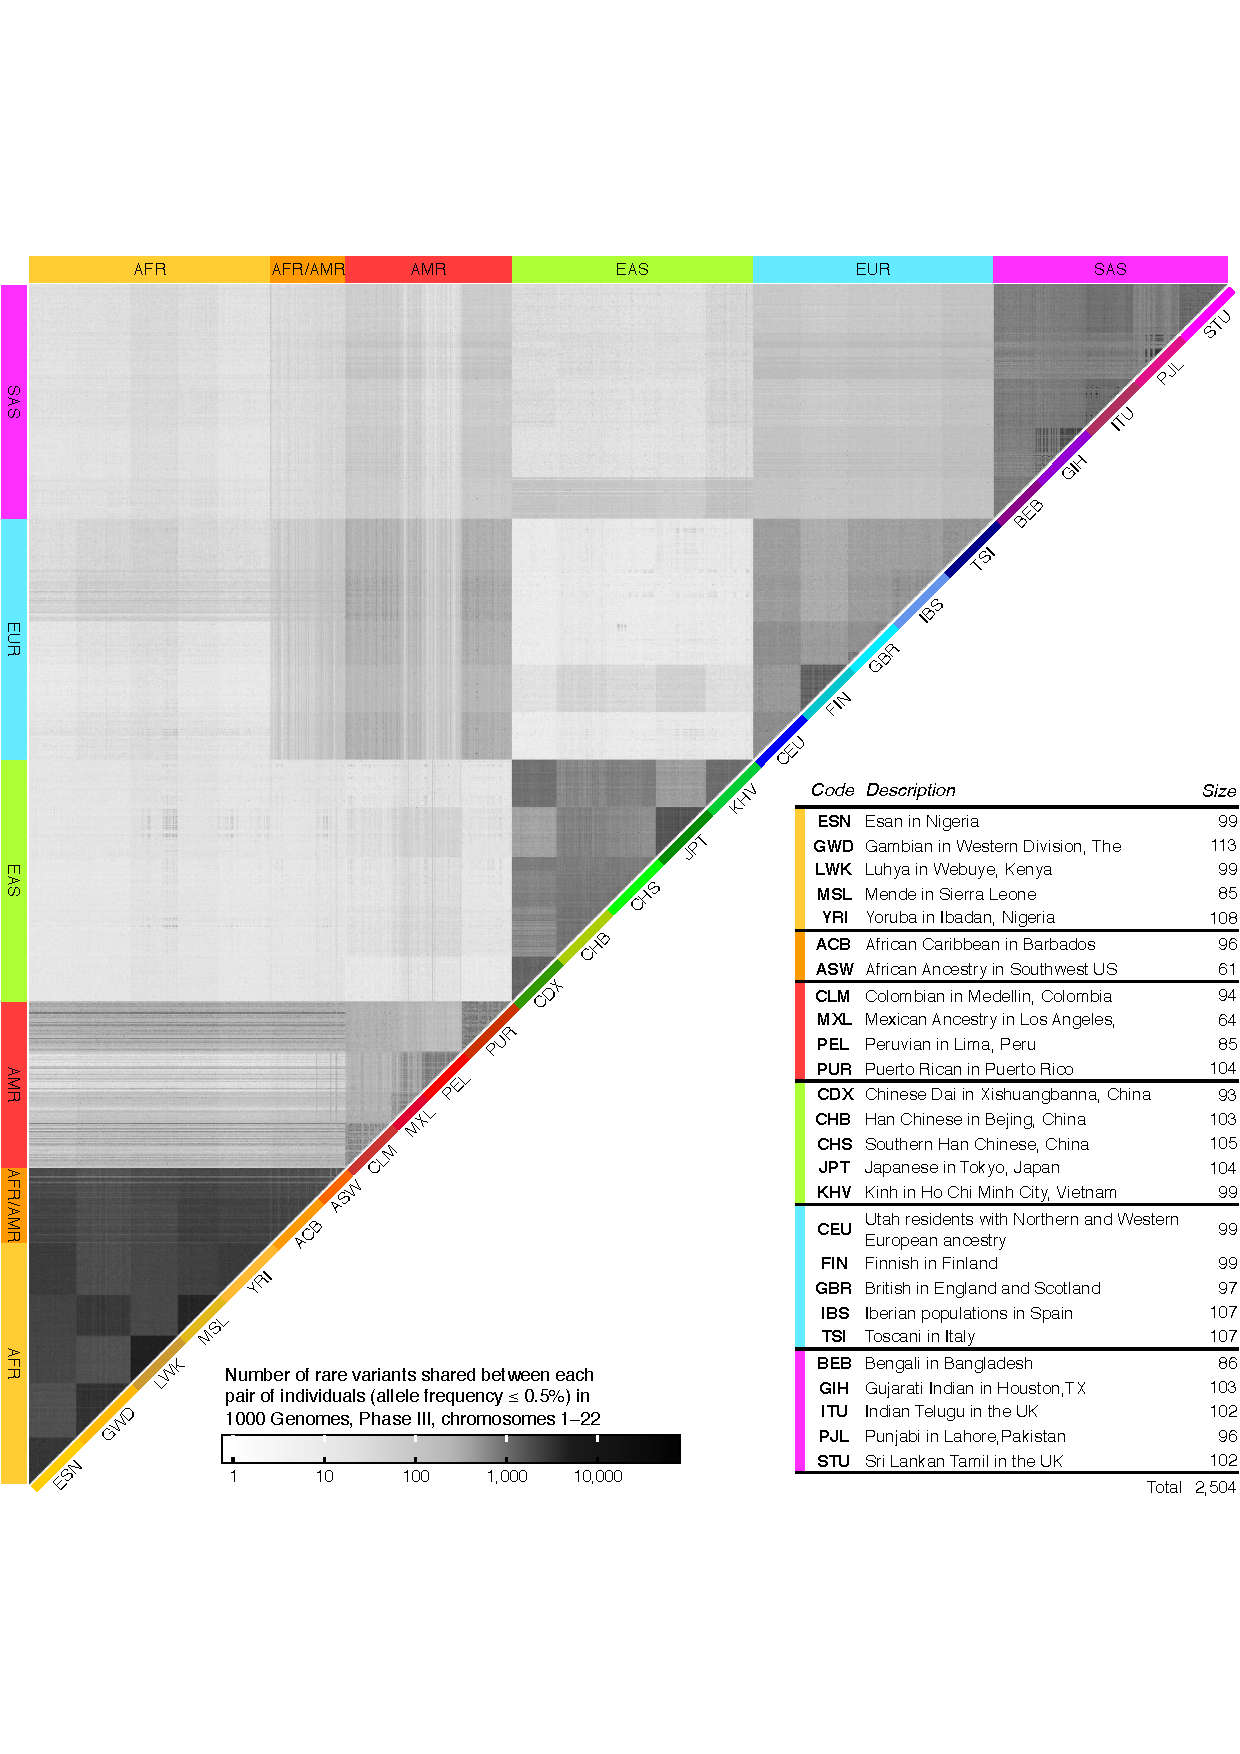
\includegraphics[width=1.1\textwidth]{./img/ch3/popstruct_1kg}%
}
\Caption{Rare variant sharing in the 1000 Genomes dataset}
{The plot shows the upper triangle of a pairwise sharing matrix in which the number of variants shared in each pair of individuals is indicated by tones of grey (log-scaled), ranging from \emph{light} (low number) to \emph{dark} (high number); see legend.
Pairwise rare variant sharing was determined for all shared alleles observed at  frequency ${\leq 0.5\%}$, across chromosomes 1--22, and in each pair of the \n{2504} individuals present in the final release dataset of the \glsentrylong{1kg} Phase~\rom{3}.
The dataset comprises sample data from \n{6} continental populations (or \emph{super-populations}) which are further subdivided in \n{26}~populations of different ethnic background.
Each group is abbreviated using a \n{3}-letter code.
The \n{6} continental populations are defined as follows;
African~(AFR), African-American~(AFR/AMR), American~(AMR), East~Asian~(EAS), European~(EUR), and South~Asian~(SAS).
The table in the lower right corner shows the code and description of each  population sample, as well as the number of individuals in each group.}
{fig:popstruct_1kg}
\end{figure}

%


%
%!TEX root = ../../main.tex


\begin{figure}[p]
\centering
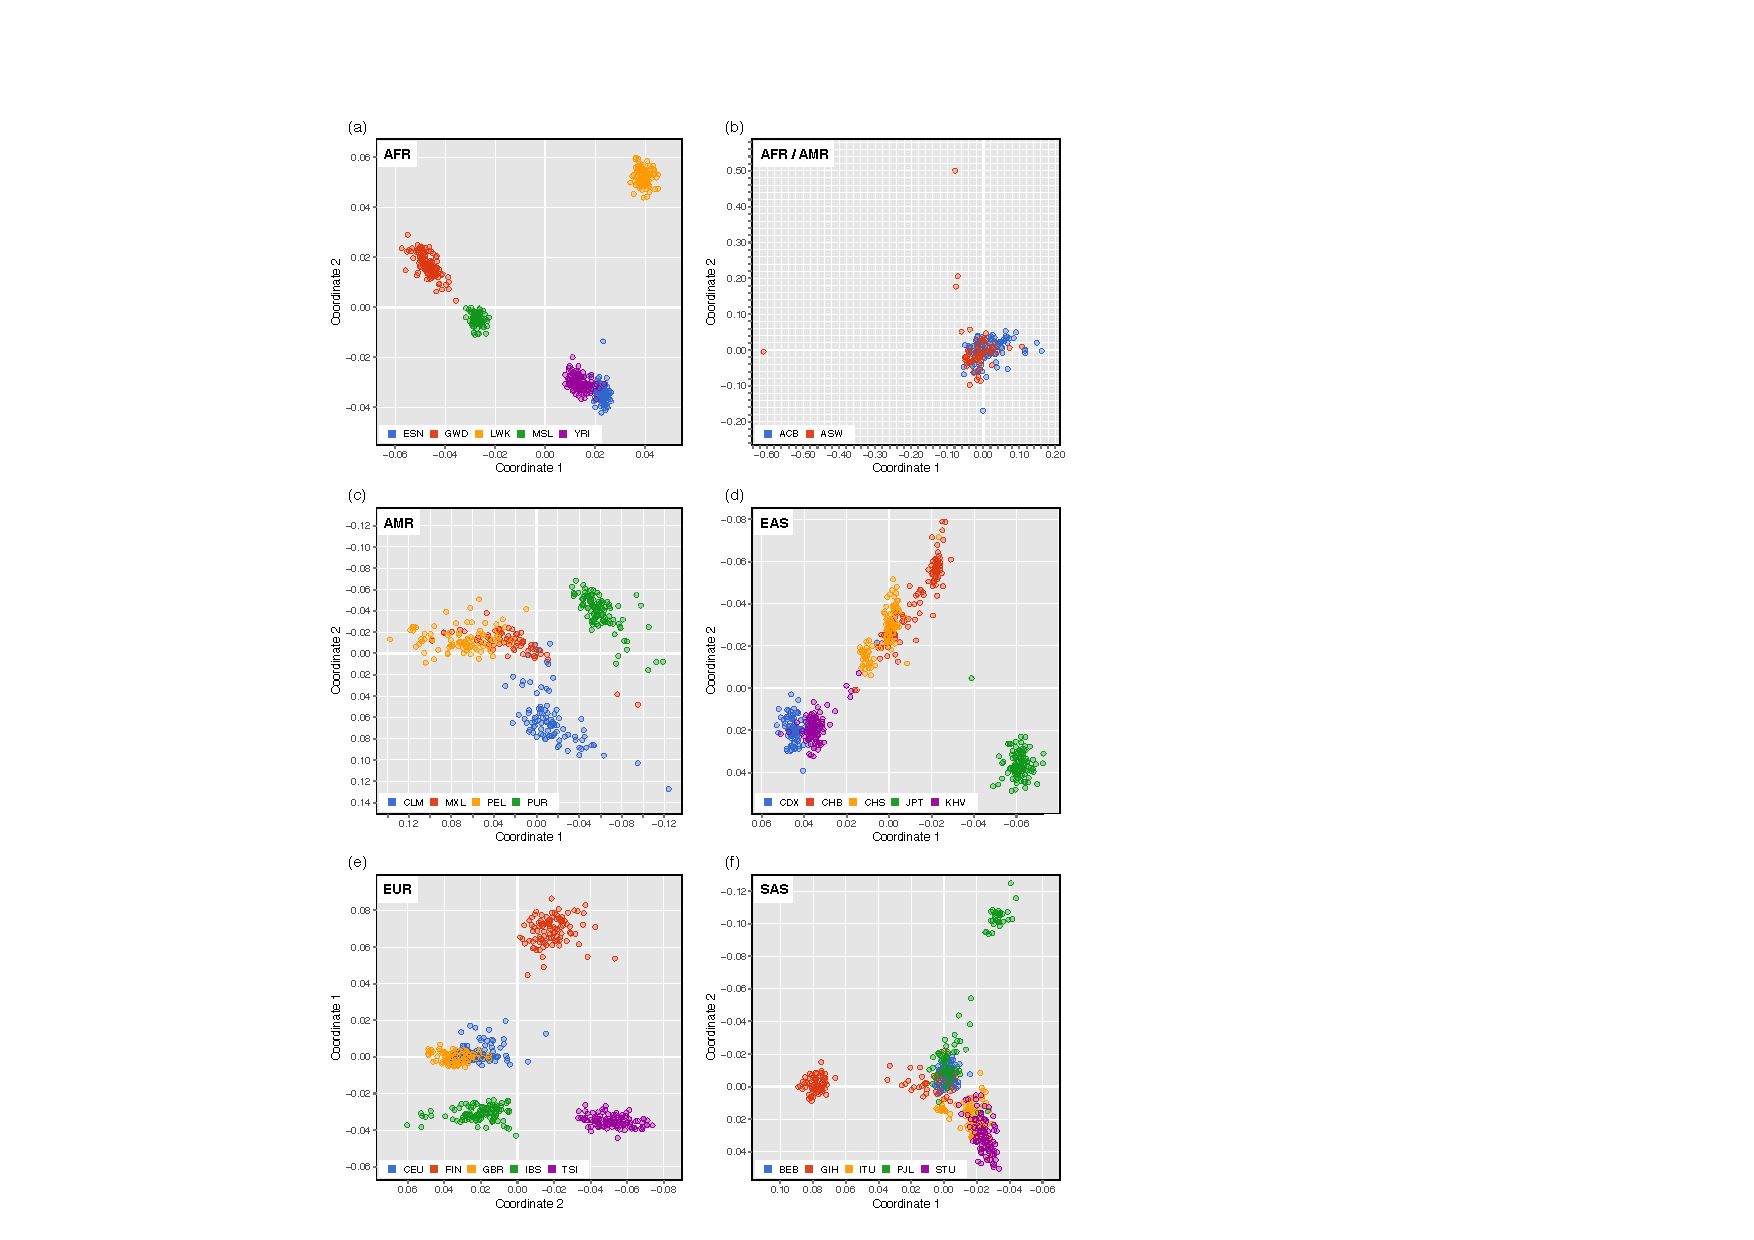
\includegraphics[width=0.9\textwidth]{./img/ch3/pcoa_1kg}
\Caption{Principal coordinates analysis of pairwise shared rare variants}
{...

Axis orientation in each panel was chosen to better reflect the cardinal directions on a geographic map; \ie the top, bottom, left and right sides of each panel roughly correspond to North, South, West, and East, respectively.
Note that the colours used do not adhere to the colour-scheme defined in the \glsentrylong{1kg}; instead, arbitrary colours were chosen to better distinguish population groups.

...}
{fig:pcoa_1kg}
% \vspace{-5pt}
% \hrulefill%
\end{figure}

%



%
\subsection{Distribution of shared haplotype lengths}
%

Overall median length was 0.158~Mb and 0.280~Mb for the \gls{fgt} and \gls{dgt}, respectively, which was considerably shorter than the median lengths detected over the same allele frequency range in simulated data, which were \gap\ and \gap{}, respectively.
This is listed in more detail in \cpref{tab:lengthrate}, in which estimated physical and genetic lengths are given per chromosome.
From those, the average recombination rate was calculated as the ratio of genetic and physical distance.

%
% !TEX root = ../../main.tex


\begin{table}[!htbp]
\Caption{Median shared haplotype lengths and inferred recombination rates by chromosome in 1000 Genomes data}
{Shared haplotype segments in \gls{1kg} (phase~3) were inferred using the \gls{fgt} and \gls{dgt}, on data from \n{2504} individuals across all autosomes.
Pairwise shared segments were identified from rare variants at allele frequency $\leq 0.5\%$ (\fk{[2,25]}).
Median genetic and physical lengths over all inferred segments were calculated per chromosome, after removing boundary cases and retaining unique segments only.
Recombination rate is reported as the average ratio of inferred genetic and physical lengths per segment.}
{tab:lengthrate}
\centering
\begin{tabularx}{\textwidth}{c *{4}{Y} cc} \toprule
Chromosome & \multicolumn{2}{c}{Physical length (Mb)} & \multicolumn{2}{c}{Genetic length (cM)} & \multicolumn{2}{c}{Mean cM/Mb (±SE)} \\ \cmidrule(lr){2-3} \cmidrule(lr){4-5} \cmidrule(lr){6-7}
 & FGT & DGT & FGT & DGT & FGT & DGT \\ \midrule
1  & 0.170 & 0.316 & 0.186 & 0.360 & 1.559 (0.003) & 1.506 (0.002) \\
2  & 0.188 & 0.337 & 0.181 & 0.342 & 1.419 (0.003) & 1.368 (0.002) \\
3  & 0.193 & 0.332 & 0.191 & 0.347 & 1.466 (0.003) & 1.423 (0.002) \\
4  & 0.192 & 0.334 & 0.187 & 0.342 & 1.441 (0.003) & 1.397 (0.002) \\
5  & 0.195 & 0.334 & 0.194 & 0.350 & 1.478 (0.003) & 1.421 (0.002) \\
6  & 0.187 & 0.325 & 0.184 & 0.336 & 1.442 (0.003) & 1.395 (0.002) \\
7  & 0.165 & 0.292 & 0.175 & 0.327 & 1.521 (0.003) & 1.478 (0.002) \\
8  & 0.167 & 0.288 & 0.176 & 0.324 & 1.552 (0.003) & 1.508 (0.003) \\
9  & 0.150 & 0.264 & 0.197 & 0.357 & 1.857 (0.004) & 1.797 (0.003) \\
10 & 0.156 & 0.277 & 0.191 & 0.354 & 1.704 (0.004) & 1.659 (0.003) \\
11 & 0.175 & 0.306 & 0.180 & 0.334 & 1.525 (0.003) & 1.476 (0.003) \\
12 & 0.172 & 0.301 & 0.200 & 0.372 & 1.710 (0.004) & 1.648 (0.003) \\
13 & 0.172 & 0.295 & 0.202 & 0.362 & 1.675 (0.004) & 1.613 (0.003) \\
14 & 0.164 & 0.287 & 0.190 & 0.353 & 1.719 (0.004) & 1.664 (0.003) \\
15 & 0.136 & 0.243 & 0.185 & 0.358 & 2.080 (0.005) & 2.036 (0.004) \\
16 & 0.110 & 0.205 & 0.175 & 0.344 & 2.288 (0.005) & 2.244 (0.004) \\
17 & 0.128 & 0.237 & 0.179 & 0.350 & 2.118 (0.005) & 2.060 (0.004) \\
18 & 0.149 & 0.254 & 0.203 & 0.368 & 2.011 (0.005) & 1.934 (0.004) \\
19 & 0.105 & 0.192 & 0.176 & 0.344 & 2.365 (0.005) & 2.325 (0.004) \\
20 & 0.135 & 0.231 & 0.217 & 0.395 & 2.277 (0.005) & 2.203 (0.004) \\
21 & 0.116 & 0.214 & 0.195 & 0.361 & 2.185 (0.005) & 2.100 (0.004) \\
22 & 0.094 & 0.175 & 0.172 & 0.339 & 2.693 (0.006) & 2.624 (0.005) \\
\bottomrule
\end{tabularx}
\end{table}

%

The following results provide a more direct comparison to the simulated dataset in \cpref{sec:evalsimdata}.
Because simulated data were generated using recombination rates observed in human chromosome 20, the distribution of inferred physical and genetic lengths for \gls{1kg} chromosome~20 is shown in \cpref{fig:1kg20_lengths}.
Surprisingly, both the physical and genetic lengths appeared to be uniformly distributed \Gap{}.
Also, the median length of segments detected around \fk{2} variants was shorter than expected.
Regardless, segments detected using the \gls{dgt} were longer on average than those detected using the \gls{fgt}, which was consistent with expectations.
This pattern was consistent among all chromosomes (data not shown).


%
%!TEX root = ../../main.tex


\begin{figure}[!htbp]
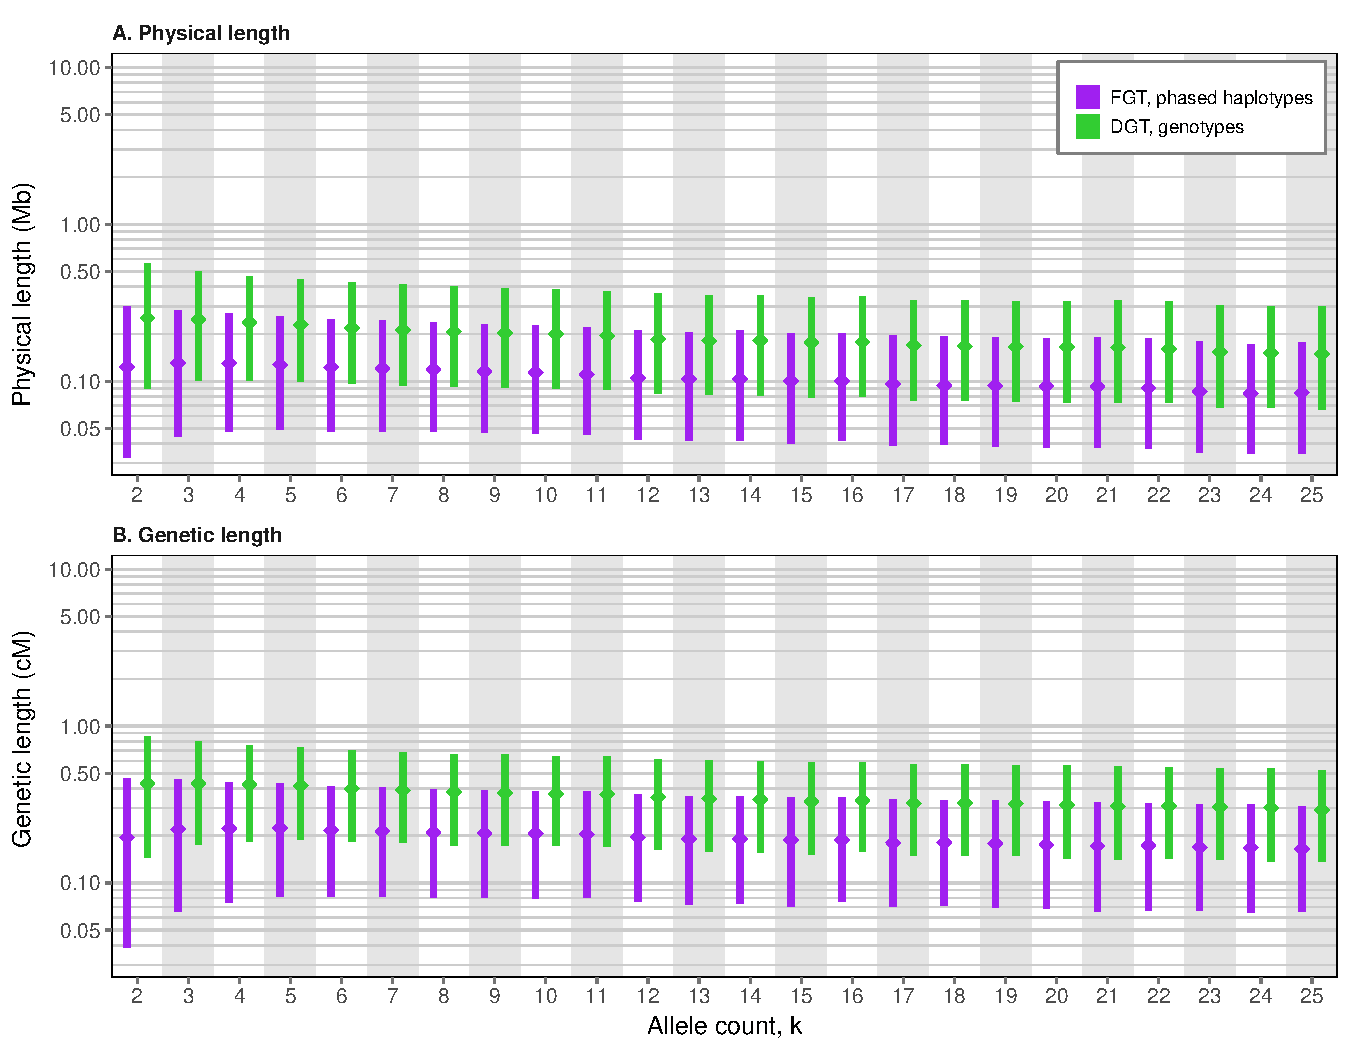
\includegraphics[width=\textwidth]{./img/ch3/length_1kg20}
\Caption{Distribution of inferred IBD lengths in 1000 Genomes data, chromosome 20}
{Results are shown for the detected physical and genetic lengths of shared haplotype segments by \fk{}, using chromosome 20 in the final release dataset of \glsentrylong{1kg} Phase~\rom{3}, including ${N = \num{2504}}$ individuals.
IBD segments were detected using the \gls{fgt} (on phased haplotypes) and the \gls{dgt} (on genotype data).
Bottom and top of each bar represent the \nth{1} and \nth{3} quartile, respectively, between which the median (\nth{2} quartile) is marked (\emph{diamonds}).}
{fig:1kg20_lengths}
\end{figure}

%


% The observation that segment lengths are far from being exponentially distributed is disturbing, as it suggests that
% On the assumption that \glsfull{1kg} data is


%
\section{Discussion}
%


graph-based method
was abandoned after it became clear that
computational complexity of a graph generated for even a modest number of sharers
high redundancy
reduced flexibility

Nonetheless, it is an intriguing idea to represent all possible paths in a graph-like structure
initially constructing ``vertical'' trees branching along the length of a chromosome and growing to both sides of a given target position.
for example, as a method to reconstruct the most likely sequence of marginal trees along the length of a chromosome; \ie to
\gls{arg}
An initial concept of this idea was implemented in \cpp and evaluated on a small number of rare variants.
However, the concept was abandoned due to \n{3} reasons.
First,

Thus, further research would be required to address these issues and make such an approach computationally tractable.
Second, the information that could be captured by a graph-based method does not offer any advantage over an exhaustive pairwise approach (as presented in this chapter).
While it is likely that an IBD graph would
\eg for the purpose of genomic data compression
from which pairwise IBD information could be retrieved
Furthermore, there already is a
The pairwise detection of IBD segments is therefore implicitly faster
Third, the inference process of the IBD graph would suffer from deviations of model assumptions (in particular the infinite sites model) as well as genotype error,
more so than than the presented pairwise approach due to the incremental construction and reciprocal connection of the graph which relies on


% The length distribution of shared haplotype tracts is shown in \cref{fig:1kg_lengths}.
% Over all detected segments in \fk{[2, 25]}, median genetic length was 0.19~cM and 0.36~cM for \gls{fgt} and \gls{dgt}, respectively.
% Likewise, median physical length was 0.15~Mb and 0.27~Mb for \gls{fgt} and \gls{dgt}, respectively.




redundant information



A full-fledged application based on available IBD information alone is less commendable due to several reasons; see below.

\begin{itemize}
	\item

	\item The constraints imposed by the genealogy are not conclusive.
	For example, if the genotypes in both individuals are heterozygous at a given site, it cannot be determined whether the allele sits on the same haplotype as the alleles at other double-heterozygous sites, \eg such as the alleles at the target position around which the IBD segment was inferred.

	\item The underlying IBD segment is expected to be fully enclosed within the detected breakpoint interval, but where the genealogy may not be consistent over the full length of the segment.
	Due to overestimation, it is expected that phasing becomes erroneous towards the terminal ends of a segment.
\end{itemize}



Idea: use FGT and DGT to derive an expectation for the rate of phasing and genotype errors in real data.
FGT is ``tripped'' by
